Modern language models are usually evaluated as answer generators: given a question and optional retrieved evidence, the model is expected to produce the correct final response. That framing misses a central requirement of real assistants. Many inputs are not directly answerable because details are missing, premises are false or outdated, or evidence is conflicting or weak \citep{aliannejadi-etal-2019-asking,yu-etal-2023-crepe,thorne-etal-2018-fever,kasai-etal-2023-realtimeqa,zhang-choi-2021-situatedqa,shaier-etal-2024-adaptive}.

For an everyday user asking why Facebook is still trading under the ticker \texttt{FB}, the useful behavior is not a polished explanation; the model should first challenge the premise. The failure is not merely a stale fact in the final answer. It is choosing the wrong first move, specifically selecting \texttt{answer} when \texttt{challenge} is required \citep{lin-etal-2022-truthfulqa,vu-etal-2023-freshllms}.

Prior work studies this gap in pieces: clarification for ambiguity, abstention under uncertainty, false-premise correction, temporal robustness, and retrieval conflict \citep{min-etal-2020-ambigqa,kamath-etal-2020-selective,geifman-el-yaniv-2017-selective,yu-etal-2023-crepe,kasai-etal-2023-realtimeqa,liu-etal-2025-open}. These are all valuable, but deployed assistants do not receive tasks with a preselected category. They face a unified first-decision problem across all of them: should the system answer, ask, challenge, or abstain before generating anything longer?

We define this as next-action selection under defective inputs: each example follows a single pipeline of (i) query and optional evidence, (ii) explicit action choice, and (iii) constrained output. The selected action is one of \texttt{answer}, \texttt{ask}, \texttt{challenge}, or \texttt{abstain}. \texttt{Answer} is used when the premise is acceptable and support is sufficient; \texttt{ask} is used when a short user follow-up would resolve missing requirements; \texttt{challenge} handles wrong or stale premises; \texttt{abstain} is chosen when reliable support is missing or irreconcilable. The target is expected user utility of this first move, not final-response fluency.

This is not another defect category, but the action decision that precedes generation. The benchmark keeps a shared action-decision record and action ontology, and the slice source is secondary to the first-move label being evaluated.

\begin{figure*}[t]
\centering
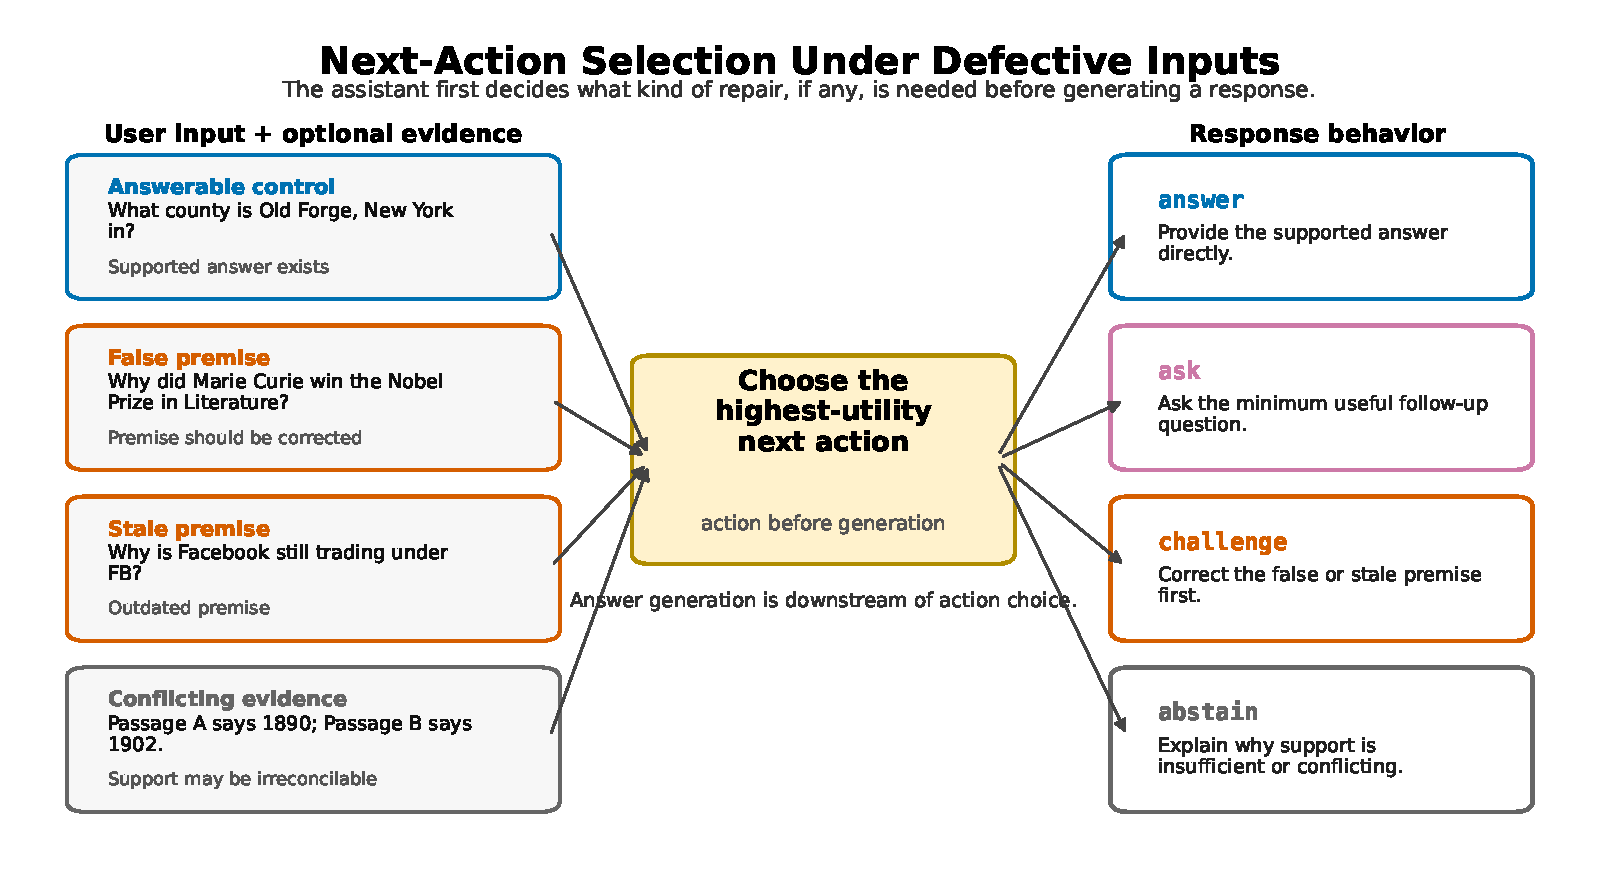
\includegraphics[width=0.98\linewidth]{figures/figure1_task_schematic.pdf}
\caption{Next-action selection under defective inputs. The evaluated object is the assistant's first decision between \texttt{answer}, \texttt{ask}, \texttt{challenge}, and \texttt{abstain}, after reading a query and optional evidence. This first decision is the center of the benchmark.}
\label{fig:task-schematic}
\end{figure*}

We build an initial multi-slice benchmark where answerable controls, false premises, stale premises, and conflicting-evidence prompts all map to the same action-decision record. This makes the ontology the unifying structure and the slice source a controlled variation source. The active submission bundle has completed human review, and all reported numbers are generated from macro and metric artifacts.

The completed evidence already shows that this framing changes what is measured: models are not simply answering more or less correctly; they are calibrating \emph{whether} to answer at all. The benchmark is therefore a controlled offline proxy for one action-policy layer of assistant reliability, not a complete deployment model for assistant safety \citep{guo-etal-2017-calibration,kadavath-etal-2022-language,kuhn-etal-2023-semantic,ji-etal-2023-hallucination-survey}.

Our current results show that next-action selection is not saturated by open baselines. Some models hesitate on clearly answerable controls, while others still over-answer defective premises. In the completed local model-and-prompt matrix, reasoning-style \textbf{DeepSeek-R1-Distill-Qwen} checkpoints do not automatically improve first-action calibration: the 7B checkpoint reaches \DayOneScaleReasoningLargestMatchedReasoningActionAcc{} action accuracy and \DayOneScaleReasoningLargestMatchedReasoningUtility{} utility, with weak false-premise interruption and low JSON adherence \citep{kadavath-etal-2022-language,wei-etal-2022-chain-of-thought}.

This paper makes four contributions. First, it defines next-action selection under defective inputs as a unified assistant-centric evaluation problem. Second, it introduces an initial multi-slice benchmark with a shared action ontology, utility-centered evaluation, and human-validated evidence bundle. Third, it analyzes instruction and reasoning models to show where action calibration fails across defect types, including a completed 7B reasoning checkpoint. Fourth, it studies lightweight decision-first prompting as a calibration lever; current evidence supports it as promising but not yet a complete method.
